\chapter{Implementação}
% Os titulos dados aos capítulos são meros exemplos. Cada relatório deve adequar-se ao projeto desenvolvido.
\label{chap:imp-test}

\section{Introdução}
\label{chap4:sec:intro}

Neste capítulo abordamos a implementação de cada um dos objectivos realizados no trabalho. Visto o foco deste trabalho ser a Segurança Informática, deixamos de parte outras implementações menos focadas no objetivo, como por exemplo, o \textit{Design}. \newline Abordamos também neste capitulo, um Manual de utilização do programa. \newline Também, por não ser o nosso foco, decidimos não dedicar muito tempo ao tratamento de pequenos erros (como o \textit{input} de \textit{nicknames} iguais) que poderão dar problemas.
\newline Neste capítulo cada secção intermédia irá representar um dos pontos dos objectivos do trabalho prático e discutirá a sua implementação .

\newline\section{Geração de um segredo criptográfico a partir de palavras-passe inseridas pelo utilizador, nomeadamente através de algoritmos como o Password \textit{Based Key Derivation Function 2} (PBKDF2)}
\label{chap4:sec:pbkdf}

O trecho de código seguinte corresponde a uma pedaço do ficheiro \texttt{D\_PBKDF2} correspondente à geração do criptograma:
\begin{lstlisting}[caption=Trecho de código usado no projeto.]
    String password = palavra.getText();
    String secret = segredo.getText();
    int option = box.getSelectedIndex() + 1;
    
    PBKDF2 pbkdf2 = new PBKDF2(password, option);
    String criptogram = pbkdf2.encrypt(secret);
    
    JOptionPane.showMessageDialog(this,
        "Criptograma gerado: \n" + criptogram,
        "Informação",
    JOptionPane.INFORMATION_MESSAGE);
\end{lstlisting}
O trecho de código seguinte corresponde a um trecho da classe \texttt{PBKDF2} usada para a realização deste algoritmo.
\begin{lstlisting}[caption=Trecho de código usado no projeto.]
    Cipher dcipher;

    byte[] random = getRandom();
    int iterationCount = 1024;
    int keyLength = 128;  //tamanho da chave
    SecretKey key;
    byte[] iv;
    
    public PBKDF2(String passPhrase, int opcao_hash) throws Exception {
        SecretKeyFactory factory = null;
        switch (opcao_hash) {
            case 1: {        //SHA1
                factory = SecretKeyFactory.getInstance("PBKDF2WithHmacSHA1");
                break;
            }
            case 2: {        //SHA224
                factory = SecretKeyFactory.getInstance("PBKDF2WithHmacSHA224");
                break;
            }
            case 3: {        //SHA256
                factory = SecretKeyFactory.getInstance("PBKDF2WithHmacSHA256");
                break;
            }
            case 4: {        //SHA384
                factory = SecretKeyFactory.getInstance("PBKDF2WithHmacSHA384");
                break;
            }
            case 5: {        //SHA512
                factory = SecretKeyFactory.getInstance("PBKDF2WithHmacSHA512");
                break;
            }
        }

        KeySpec spec = new PBEKeySpec(passPhrase.toCharArray(), random, iterationCount, keyLength);
        SecretKey temp = factory.generateSecret(spec);
        key = new SecretKeySpec(temp.getEncoded(), "AES");
        dcipher = Cipher.getInstance("AES/CBC/PKCS5Padding");
    }

    public String encrypt(String data) throws Exception {
        dcipher.init(Cipher.ENCRYPT_MODE, key);
        AlgorithmParameters params = dcipher.getParameters();
        iv = params.getParameterSpec(IvParameterSpec.class).getIV();
        byte[] utf8EncryptedData = dcipher.doFinal(data.getBytes());
        String base64EncryptedData = Base64.getEncoder().encodeToString(utf8EncryptedData);
        return base64EncryptedData;
    }
    
    //gera aleatório
    private static byte[] getRandom() throws NoSuchAlgorithmException { 
        SecureRandom sr = SecureRandom.getInstance("SHA1PRNG");
        byte[] random = new byte[16];
        sr.nextBytes(random);
        return random;
    }
\end{lstlisting}

Gerar segredo criptográfico através de chave gerada por palavra-passe \\ (PBKDF2): Esta função vai cifrar um segredo com o auxílio de uma palavra-passe, onde o cliente pode escolher entre várias funções de \emph{hash}. 

Com a palavra-passe introduzida, o programa irá pegar na mesma, em \codigo\textit{{salt}}, no número de iterações que terá de executar e no tamanho da chave. O \codigo\textit{{salt}} em conjunto com a palavra-passe utilizada irá gerar um novo vetor de \emph{bytes}. Através disso e com a chave secreta que foi gerada com o auxílio da função de \textit{hash}, vai calcular uma nova chave (com o algoritmo AES). Após isso, usa a chave gerada anteriormente e pega na mensagem, encriptando a mesma com "AES/CBC/PKCS5Padding" usando o vetor de inicialização e transforma este conjunto de \emph\textit{{bytes}} em \textit{base64} para assim ser percetível ao utilizador.

\newline\section{Troca de um segredo criptográfico usando o protocolo de acordo de chaves \textit{DiffieHellman}}
\label{chap4:sec:diffiehellman}

O trecho de código seguinte mostra um pedaço da função \texttt{sendSecret()} correspondente à parte onde este o algortimo para a execução deste ponto é invocado pela Alice. 
\begin{lstlisting}[caption=Trecho de código usado no projeto.]  
    SecureRandom rnd = new SecureRandom();
    BigInteger P, G, x, X, Y, K;
    
    boolean b;
    do {
        P = BigInteger.probablePrime(1024, rnd);
        b = P.isProbablePrime(100);
    } while(!b);
    System.out.println("Generated P: " + P.toString());
    
    G = DiffieHellman.nextRandomBigInteger(P);
    System.out.println("Generated G: " + G.toString());
    
    x = DiffieHellman.nextRandomBigInteger(P);
    System.out.println("Generated x: " + x.toString());
    
    X = G.modPow(x, P);  // X = G^x mod P
    
    out.writeObject(P);
    out.flush();
    out.writeObject(G);
    out.flush();
    out.writeObject(X);
    out.flush();
            
    Y = (BigInteger) in.readObject();
    
    K = Y.modPow(x, P);
    
    String criptograma = AES.encrypt(message, K.toString());
    out.writeObject(criptograma);
    out.flush();
\end{lstlisting}
O seguinte techo correponde à parte do Bob.
\begin{lstlisting}[caption=Trecho de código usado no projeto.]
    P = (BigInteger) in.readObject();
    G = (BigInteger) in.readObject();
    X = (BigInteger) in.readObject();

    y = DiffieHellman.nextRandomBigInteger(P);

    Y = G.modPow(y, P);  // X = g^x mod p
    
    out.writeObject(Y);
    out.flush();
    
    K = X.modPow(y, P);
    String cript = (String) in.readObject();
    message = AES.decrypt(cript, K.toString());
\end{lstlisting}

O protocolo de acordo de chaves \textit{Diffie-Hellman} serve para  partilhar um segredo sem que tenha existido uma troca de chaves prévia entre a Alice (cliente emissor) e o Bob (cliente recetor). Usando o protocolo de acordo de chaves \textit{Diffie-Hellman} um adversário (ou Claire) pode escutar a comunicação, mas não pode manipulá-la.   
\paragraph{}
Este acordo de chaves descreve-se da seguinte forma:
\begin{itemize}
    \item A Alice e o Bob escolhem um número primo fixo suficiente grande (p). Este número  pode ser tornado público. No nosso caso esse número tem 1024 \textit{bits}.
    \begin{itemize}
       \item Para realizar este passo utilizamos a função \texttt{probablePrime} que a biblioteca \texttt{java.math.BigInteger} nos disponibiliza, e assim obtemos um número que provavelmente é primo. O valor de retorno tem uma probabilidade de não ser primo de $2^{-100}$. Este valor vai ainda ser confirmado dentro de um ciclo \codigo\textit{{do while}} que fica a correr enquanto a função \texttt{isProbablePrime} confirma se o numero p é mesmo número primo. Esta função é disponibilizada pela biblioteca referida acima.
    \end{itemize}
    \item De seguida, é definido um gerador g entre 1 e p que pode ser tornado publico.
       \begin{itemize}
           \item Gera-se este valor fazendo uma chamada à função \texttt{nextRandomBigInteger} que se encontra na classe \texttt{DiffieHelman}.
       \end{itemize}
    \item Quando estes dois valores (p e g) são combinados entre ambos, a Alice escolhe um numero x entre 1 e p, que irá ser a sua chave secreta, e calcula $X=g^x \bmod p$ e envia X ao Bob. X pode ser público.
    \item O Bob recebe X e  escolhe um número y , que irá ser a sua chave secreta, entre 1 e p e calcula $Y=g^y \bmod p$ e envia Y para a Alice, o valor Y pode ser tornado público.
    \item Quando a Alice tiver o Y calcula k da seguinte forma: $k= Y^x \bmod p$. k será a chave secreta que ambos vão ter. O Bob calcula k recorrendo a $k=X^y\bmod p$.
\end{itemize}
\paragraph{}
Depois usando o AES encripta-se a mensagem é envia ao outro utilizador, que por sua vez já terá a chave k para poder desencriptar e ler a mensagem.

\newline\section{Troca de um segredo criptográfico usando \textit{Puzzles} de \textit{Merkle}}
\label{chap4:sec:merkle}

O trecho de código seguinte mostra um pedaço da função \texttt{sendSecret()} correspondente à parte onde este o algortimo para a execução deste ponto é invocado pela Alice. 

\begin{lstlisting}[caption=Trecho de código usado no projeto.]
    MerklePuzzle mp = new MerklePuzzle();
    int totalPuzzles = 10000;
    int keyLen = 4;
    
    ArrayList<byte[]> puzzles = new ArrayList<>();
    ArrayList<String> keys = new ArrayList<>();
    for (int i = 0; i < totalPuzzles; i++) {
        String aux = mp.random_string(16);
        keys.add(i, aux);
        byte[] cipherText = mp.encrypt(mp.random_key(keyLen), (aux + "PUZZLE" + i));
        puzzles.add(cipherText);
    }
    
    Collections.shuffle(puzzles);
    
    out.writeObject(puzzles);
    out.flush();
    out.writeObject(MerkleCipher);
    out.flush();
    out.writeInt(keyLen);
    out.flush();
    
    String chosen = (String) in.readObject();
    
    String keyChosen = keys.get(Integer.parseInt(chosen)); // chave simétrica
    byte[] encriptedMessage = null;
    
    if (MerkleCipher.equalsIgnoreCase("AES-ECB")) {
        
        byte[] encodedKey = keyChosen.getBytes();
        SecretKey sk = new SecretKeySpec(encodedKey, 0, encodedKey.length, "AES");
    
        encriptedMessage = AES.encrypt(message, sk);
        
    } else {
        
        String keyZ = keyChosen + keyChosen;
        byte[] temp = keyZ.getBytes(Charset.forName("UTF-8"));
        SecretKey sk = new SecretKeySpec(temp, 0, 8, "DES");
        
        encriptedMessage = DES.encrypt(message, sk);
        
    }
    
    out.writeObject(encriptedMessage);
    out.flush();
\end{lstlisting}
O seguinte techo correponde à parte do Bob.
\begin{lstlisting}[caption=Trecho de código usado no projeto.]
    MerklePuzzle mp = new MerklePuzzle();
                    
    ArrayList<byte[]> puzzles = (ArrayList) in.readObject();
    cipherMode = (String) in.readObject();
    int keyLen = in.readInt();
    
    int chosen = new SecureRandom().nextInt(puzzles.size());
    String tempKey = "";
    boolean solved = false;
    while(!solved) {
        tempKey = mp.decrypt(mp.random_key(keyLen), puzzles.get(chosen));
        
        if (tempKey != null && tempKey.contains("PUZZLE"))
            solved = true;
    }
    
    System.out.println("TotalPuzzles= " + puzzles.size());
    System.out.println("Key= " + tempKey.substring(0, 16) + "\nPuzzle= " + tempKey.substring(22));
    
    String key = tempKey.substring(0, 16);

    out.writeObject(tempKey.substring(22));
    out.flush();
    
    byte[] encodedKey = key.getBytes();
    
    byte[] criptogram = (byte[]) in.readObject();
    
    if (cipherMode.equalsIgnoreCase("AES-ECB")) {
        SecretKey sk = new SecretKeySpec(encodedKey, 0, encodedKey.length, "AES");
        message = AES.decrypt(criptogram, sk);
    } else {
        String keyZ = key + key;
        byte[] temp = keyZ.getBytes(Charset.forName("UTF-8"));
        SecretKey sk = new SecretKeySpec(temp, 0, 8, "DES");
        
        message = DES.decrypt(criptogram, sk);
    }
\end{lstlisting}
Neste algoritmo a Alice cria os puzzles cada um com chaves diferentes.(Excerto de Código 4.5) Cada \textit{puzzle} é encriptado usando o algoritmo de cifra DES com uma chave aleatória diferente (Cada chave gerada é guardada numa lista que só Alice tem acesso). Depois dos \textit{puzzles} serem gerados são baralhados e enviados para o Bob.(Excerto de código 4.6) Depois dos puzzles serem enviados ao Bob, ele escolhe um aleatoriamente e tenta decifrá-lo. Quando consegue decifrar fica a saber o número do \textit{puzzle} e uma chave. O Bob envia então para a Alice o número do puzzle que decifrou e guarda a chave.A Alice recebe o número do \textit{puzzle}, vai à sua lista que contem as chaves e vê qual a chave que esse \textit{puzzle} continha. A partir desse momento ambos têm acesso a uma chave simétrica. A Alice cifra a mensagem com o algoritmo de cifra escolhido anteriormente (AES-ECB ou DES)(Excerto de Código 4.6) e envia o criptograma gerado para o Bob que usa a chave para o decifrar e ter acesso ao segredo que lhe foi enviado.


\newline\section{Troca de um segredo criptográfico usando o Rivest, Shamir e Adleman (RSA)}
\label{chap4:sec:rsa}

O trecho de código seguinte mostra um pedaço da função \texttt{sendSecret()} correspondente à parte onde este o algoritmo para a execução deste ponto é invocado pela Alice. Ou seja vai ser pedido ao Bob que envie a sua chave publica, para a Alice assim que esta receber a chave pública vai poder encriptar a sua mensagem, através da função \texttt{encrypt()}, que está na classe \texttt{RSA}, cujo seu resultado vai ser o criptograma pronto a enviar.

\begin{lstlisting}[caption=Trecho de código usado no projeto.]
    ObjectInputStream inputStream = new ObjectInputStream(new FileInputStream((String) in.readObject()));
              
    byte[] criptograma = RSA.encrypt(message, (PublicKey) inputStream.readObject());
    out.writeObject(criptograma);
    out.flush();
\end{lstlisting}
O seguinte techo correponde à parte do Bob.
\begin{lstlisting}[caption=Trecho de código usado no projeto.]
    RSA.generateKey();
    out.writeObject(RSA.PUBLIC_KEY_FILE);
    out.flush();
    
    criptograma = (byte[]) in.readObject();
    ObjectInputStream inputStream = new ObjectInputStream(new FileInputStream(RSA.PRIVATE_KEY_FILE));
    PrivateKey privatekey = (PrivateKey) inputStream.readObject();
    message = RSA.decrypt(criptograma,privatekey);
\end{lstlisting}

Assim que o Bob receber um pedido da chave pública vai a enviar de modo a que esse utilizador consiga avançar no processo e encriptar a mensagem, depois o Bob vai receber o criptograma que é proveniente da Alice ou de outro qualquer utilizador.

\section{Distribuição de novas chaves de cifra a partir de chaves pré-distribuídas}
\label{chap4:sec:predistribuidas}

O trecho de código seguinte mostra um pedaço da função \texttt{sendSecret()} correspondente à parte da Alice. 
\begin{lstlisting}[caption=Trecho de código usado no projeto.]
    // generate new key
    MerklePuzzle mp = new MerklePuzzle();
    String randomKey = mp.random_string(20);
    
    byte[] decodedKey = Client.ins.preDistributedKey.getBytes();
    SecretKey originalKey = new SecretKeySpec(decodedKey, 0, 16, "AES");

    byte[] encryptedKey = AES.encrypt(randomKey, originalKey);

    decodedKey = randomKey.getBytes();
    originalKey = new SecretKeySpec(decodedKey, 0, 16, "AES");
    byte[] encryptedMessage = AES.encrypt(message, originalKey);
    

    out.writeObject(encryptedKey);
    out.flush();
    out.writeObject(encryptedMessage);
    out.flush();
\end{lstlisting}
O seguinte trecho corresponde à parte do Bob.
\begin{lstlisting}[caption=Trecho de código usado no projeto.]
    byte[] encryptedKey = (byte[]) in.readObject();
    byte[] encryptedMessage = (byte[]) in.readObject();
    
    
    byte[] keyByte = Client.ins.preDistributedKey.getBytes();
    SecretKey originalKey = new SecretKeySpec(keyByte, 0, 16, "AES");

    String aux = AES.decrypt(encryptedKey, originalKey);

    keyByte = aux.getBytes();
    originalKey = new SecretKeySpec(keyByte, 0, 16, "AES");

    message = AES.decrypt(encryptedMessage, originalKey);
\end{lstlisting}

Para a utilização deste ponto, trocamos um segredo a partir de uma chave pré-distribuída em ambos os Clientes. Neste método é gerada uma chave aleatória e encriptada com AES através da chave pré-distribuída e a mensagem original é encriptada usando também AES com a chave aleatória gerada. O Bob vai decifrar a chave aleatória com a chave pré-distribuída e depois decifrar a mensagem original.

\section{Implementar forma de ter a certeza de que o segredo partilhado é o mesmo dos dois lados}
\label{chap4:sec:assinaturadigital}

O trecho de código seguinte mostra um pedaço da função \texttt{sendSecret()} correspondente à parte onde está o algoritmo para a execução deste ponto é invocado pela Alice.
\begin{lstlisting}[caption=Trecho de código usado no projeto.]
    PublicKey pk = EncryptManager.getIns().getDigitalSIgnature().getMyPk();
    out.writeUTF(username);
    out.flush();
    out.writeObject(pk);
    out.flush();
   
    byte[] signedMessage = EncryptManager.getIns().getDigitalSIgnature().getSignature(message);

    out.writeObject(signedMessage);
    out.flush();
\end{lstlisting}
O seguinte trecho de código corresponde à parte do Bob.
\begin{lstlisting}[caption=Trecho de código usado no projeto.]
    String receivedUsername = in.readUTF();
    PublicKey pk = (PublicKey) in.readObject();
    
    EncryptManager.getIns().getDigitalSIgnature().receivedIdentification(receivedUsername, pk);
    byte[] signature = (byte[]) in.readObject();
    
    boolean validated = EncryptManager.getIns().getDigitalSIgnature().verifySignature(receivedUsername, message, signature);
    if (!validated) {
        Client.ins.showError("Assinatura inválida. \nO segredo não corresponde ao enviado. \nSegredo recebido: " + message);
        return;
    }
\end{lstlisting}
Para verificarmos se o segredo recebido é igual dos dois lados, a Alice envia para o Bob a sua \textit{PublicKey}, a sua Identificação e assinatura correspondente à mensagem original. O Bob irá receber isto e verificar a assinatura com a mensagem obtida depois de descodificada.
Para calcular a Assinatura Digital usamos a codificação \texttt{SHA256withRSA}.
\section{Manual de utilização}
\label{chap4:sec:manual}
Logo após iniciar o programa, será apresentada uma janela perguntando ao utilizador se pretende prosseguir em Modo Servidor ou em Modo Cliente.(Figura 1.3) 
\newline\begin{center}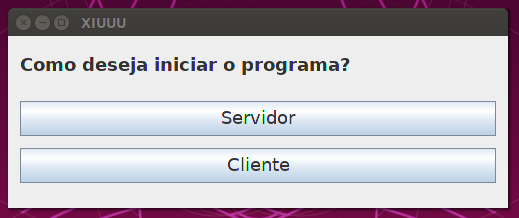
\includegraphics[scale=0.4]{img/inicio.png}\newline\caption{Figura 1.3}\end{center}
Se escolher iniciar como Servidor poderá inserir o número da porta manualmente ou manter o que se encontra por defeito (Figura 1.4).  
\newline\begin{center}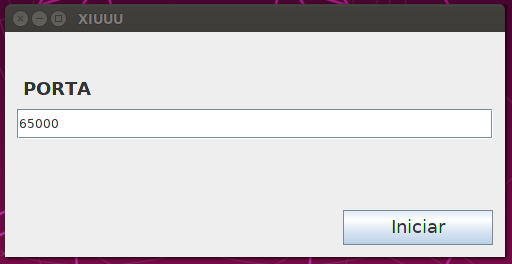
\includegraphics[scale=0.5, caption=Legenda]{img/startServer.png}\newline\caption{Figura 1.4}\end{center}
Caso pretenda optar pelo modo cliente o utilizador fará o mesmo processo como para o Servidor pois o IP está predefinido para  \textit{localhost} (Figura 1.5).
\newline\begin{center}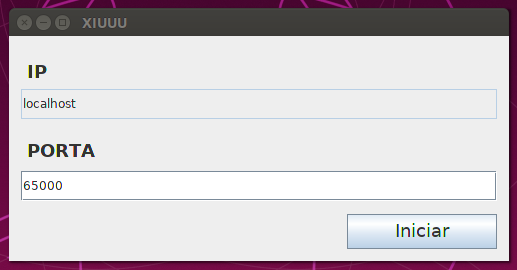
\includegraphics[scale=0.5]{img/startClient.png}\newline\caption{Figura 1.5}\end{center} 
De seguida, pode inserir o nome de utilizador que pretende (Figura 1.6)
\newline\begin{center}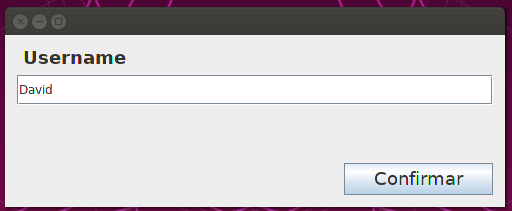
\includegraphics[scale=0.5]{img/insertUsername.png}\newline\caption{Figura 1.6}\end{center}
Depois de seleccionar o modo cliente  poderá escolher o utilizador para o qual pretende enviar um segredo ou gerar um segredo a partir de PBKDF2 (Figura 1.7).
\newline\begin{center}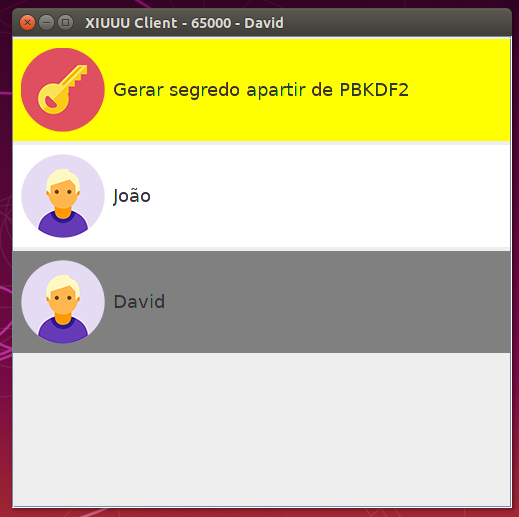
\includegraphics[scale=0.5]{img/clientInterface.png}\newline\caption{Figura 1.7}\end{center}
Após escolher gerar um segredo a partir de PBKDF2 o utilizador terá de inserir uma palavra passe, o segredo a enviar e escolher a função de \textit{hash} a utilizar (Figura 1.8).
\newline\begin{center}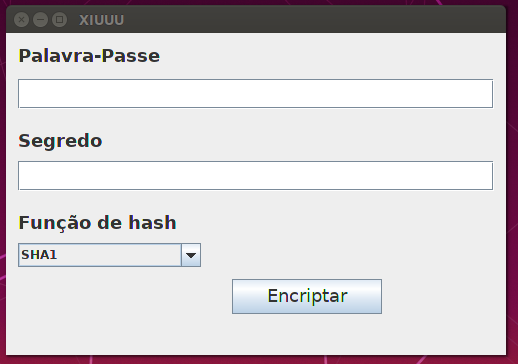
\includegraphics[scale=0.5]{img/PBKDF2.png}\newline\caption{Figura 1.8}\end{center}
Ao clicar em cliente o utilizador poderá escolher a opção de encriptação. As opções disponíveis são: RSA, \textit{DiffieHellman, MerkelPuzzle, PreDistributedKey}
\newline\begin{center}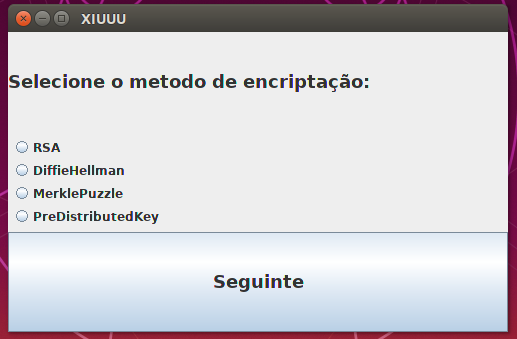
\includegraphics[scale=0.5]{img/encryptMethod.png}\newline\caption{Figura 1.9}\end{center}
Se selecionar a opção RSA,\textit{DiffieHellman} ou \textit{PreDistributedKey} (figura 1.9) será redirecionado para uma interface igual à da figura 1.10. Nesta o utilizador poderá inserir o segredo e enviá-lo. 
\newline\begin{center}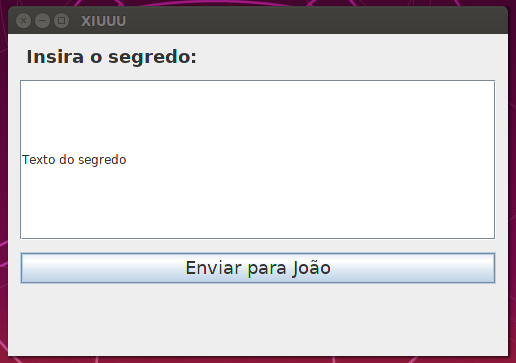
\includegraphics[scale=0.5]{img/secret.png}\newline\caption{Figura 1.10}\end{center}
Caso o utilizador deseje utilizar o método de encriptação \textit{MerklePuzzle} terá de inserir o segredo que deseja enviar e o modo de cifra. (Figura 1.11)
\newline\begin{center}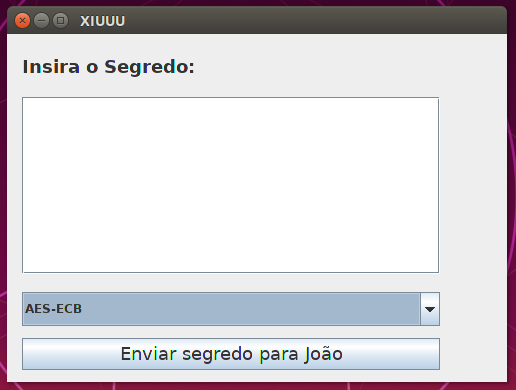
\includegraphics[scale=0.5]{img/secretMerkle.png}\newline\caption{Figura 1.11}\end{center}
Depois de ser enviado o segredo criptográfico a partir do David, o João irá receber a informação numa nova janela com os tipo de encriptação usada, o segredo e o modo de cifra. (Figura 1.12)
\newline\begin{center}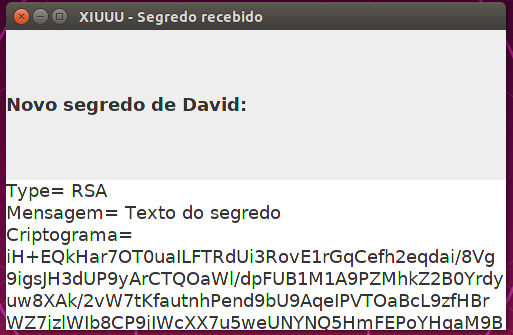
\includegraphics[scale=0.5]{img/receivedSecret.png}\newline\caption{Figura 1.12}\end{center}


\section{Conclusões}
\label{chap4:sec:concs}
Neste capítulo, estão detalhados e explicados pormenores da implementação de código, bem como justificações de decisões tomadas. Há também um manual de utilização completo, que tem o objectivo de clarificar ao máximo quem o lê, para que tenha uma melhor percepção de como utilizar a aplicação.No próximo capítulo, vão ser focados alguns problemas encontrados ao longo da construção do projecto e também reflexões sobre o estado final da aplicação.